 
\subsection{Reconfiguration of $M$}

Reconfiguring a process $M$ allows some intractable MDPs to be rendered tractable. 
As an example, take an MDP $M$ modeling a 3-dimensional foraging experiment with three thousand positions on the $x$, $y$, and $z$
axes respectively. This process will consume over three billion memory locations and may be impossible to explore. If this system is
broken into three sub problems, each targeting a special axis, then only nine thousand memory locations need be consumed. This decreases memory requirements by an exponential factor.

This section presents a method of decomposition that, when followed, introduces no degeneration of the regressed policy $\pi^{*}(s,a)$.
The summary of these conditions is presented. There is no free lunch: the trade-off for saving in space is exponentially increased computational burden. As in all problems, finding the balance between space and computational complexity is required.

 

\subsubsection{Introduction to approach}

The general approach is related to factor analysis, or clustering, eigenvalue decomposition, or projected component analysis, with which the reader may be familiar. The process is split such that a subspace $S_i \subseteq S$, and action space $A_i \subseteq A$ seem independent of subspaces $S_k$, $A_k$, for the purposes of generating reward $R(s^\prime|a,s)$. Specifically, it may be observed that the reward is homogeneous, such that 
\begin{equation*}
\forall k_2, a_2: R\left(S^\prime_i \cup  S^\prime_{k_1} \middle| S_i \cup S_{k_1} , a_i \cup a_{k_1} \right) \sim R\left( S^\prime_i \cup S^\prime_{k_2}  \middle|  S_i \cup S_{k_2} , a_i \cup a_{k_2}  \right)\,.
\end{equation*}
In this case, it is likely that the problem may be separated. Even in the case where variance of reward is high, convergence is expected.

Splitting is done using a decomposition function
\begin{equation*}
d^{M_i,M_k}_{M} = M \longrightarrow \left\{    M_i, M_k \middle|
\begin{array}{l}
S_i \times ( S_k / \{s_i\} ) = S, S_k \times ( S_i / \{ s_k \} ) = S \\
A=A_i \cup A_k\\
\tilde{T}\sim d^{-1}(d(\tilde{T})),d(\tilde{T})=\tilde{T}_i, \tilde{T}_k\\
\tilde{R}\sim d^{-1}(d(\tilde{R})), d(\tilde{R})=\tilde{R}_i,\tilde{R}_k
\end{array}
 \right\}
\end{equation*}
where $d$ represents belief mapping functions that decompose and recompose $\tilde{T}$ and $\tilde{R}$. This allows  $M$ to be mapped as new spaces and observations are encountered. The decomposition process breaks one MDP into a parent and child:\\

\begin{center}
\scalebox{0.5}{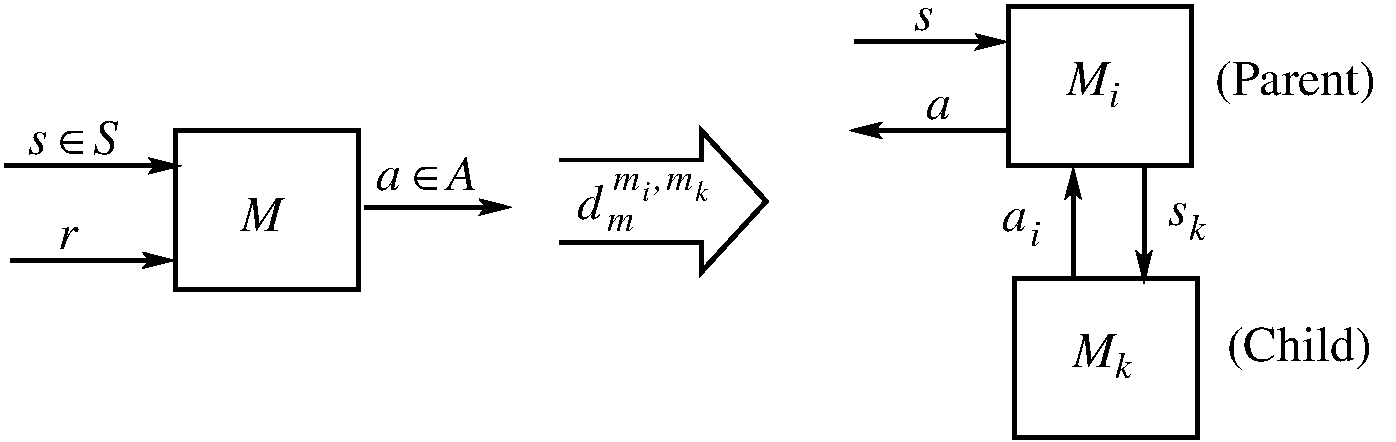
\includegraphics{media/page5figure}}
\end{center}
